\documentclass[border=5mm]{standalone}
\usepackage{pgfplots}
\pgfplotsset{compat=1.17}
\usepackage{amsmath}
\begin{document}
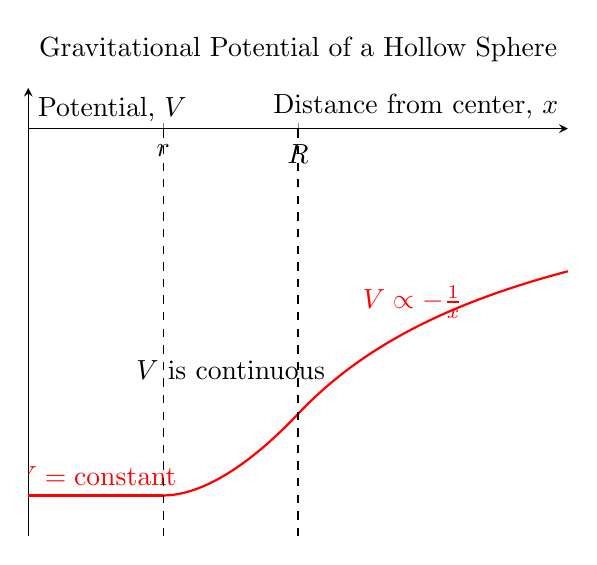
\begin{tikzpicture}
\begin{axis}[
    title={Gravitational Potential of a Hollow Sphere},
    xlabel={Distance from center, $x$},
    ylabel={Potential, $V$},
    xmin=0, xmax=4,
    ymin=-5, ymax=0.5,
    xtick={1,2},
    xticklabels={$r$, $R$},
    ytick=\empty,
    axis lines=middle,
    samples=100,
    domain=0:4
]
    % Region 1: Inside the cavity (0 <= x <= r)
    \addplot[red, thick, domain=0:1] {-4.5} node[pos=0.5, above] {$V = \text{constant}$};
    
    % Region 2: Within the material (r <= x <= R)
    \addplot[red, thick, domain=1:2] {-6 + x^2/2 + 1/x};

    % Region 3: Outside the sphere (x > R)
    \addplot[red, thick, domain=2:4] {-7/x} node[pos=0.5, above] {$V \propto -\frac{1}{x}$};

    % Dashed lines to mark r and R
    \draw[dashed] (axis cs:1,-5) -- (axis cs:1,0);
    \draw[dashed] (axis cs:2,-5) -- (axis cs:2,0);
    
    % Annotation for continuity
    \node at (axis cs:1.5, -3.2) [above] {$V$ is continuous};
\end{axis}
\end{tikzpicture}
\end{document}